\chapter{Desarrollo}

\section{Introducción}

El desarrollo del proyecto se ha estructurado en múltiples fases secuenciales, cada una diseñada para abordar aspectos específicos del proceso de análisis hiperespectral aplicado a la detección de aflatoxinas en higos frescos. La metodología desarrollada implementa técnicas de \emph{computer vision} de última generación combinadas con procesamiento especializado de datos hiperespectrales para crear un sistema automatizado de análisis de muestras.

\subsection{Adquisición de Imágenes Hiperespectrales}

Las imágenes fueron capturadas utilizando una cámara hiperespectral SPECIM, específicamente el modelo FX10 VNIR, cuyas características técnicas principales incluyen: resolución espacial de 1024 píxeles (800 \emph{width} × 1024 \emph{height}), rango espectral de 400 nm a 1000 nm (visible y parte del infrarrojo cercano), 448 bandas espectrales, y un salto espectral de 1.339 nm.

El conjunto de datos comprende 320 higos cosechados de la plantación de la variedad calabacita ubicada en la ``Finca La Orden-Valdesequera'' (38°51' N, 6°40' W, altitud 184 m) en Guadajira, España, donde CICYTEX tiene su sede central. Las imágenes hiperespectrales se capturaron durante un período de 2 semanas, utilizando cada semana 160 higos cosechados en diferentes etapas de madurez.

Cada semana, los 160 higos se dividieron en cuatro subconjuntos de 40 especímenes cada uno. El primer grupo correspondió a los controles sanos (clase 0), mientras que los tres grupos siguientes fueron inoculados con concentraciones de $10^3$ UFC/mL (clase 1), $10^5$ UFC/mL (clase 2), y $10^7$ UFC/mL (clase 3), respectivamente. El proceso de inoculación se realizó mediante inmersión del área durante aproximadamente 3 segundos, siguiendo el protocolo establecido por CICYTEX.

Las imágenes hiperespectrales se capturaron \emph{post}-inoculación cada 24 horas durante cinco días consecutivos. Entre cada sesión de adquisición, las muestras se almacenaron en una cámara de incubación controlada a 25°C, con humedad relativa entre 80 y 90\% para promover el crecimiento fúngico. Cada clase consistió de 380 imágenes hiperespectrales, generando un total de 1520 imágenes hiperespectrales para el \emph{dataset} completo.

Una vez adquiridas, las imágenes originales fueron preprocesadas con corrección blanco/negro para normalizar y corregir los datos, eliminando inconsistencias introducidas por factores ambientales, condiciones de iluminación y sensibilidad del sensor, facilitando así el análisis espectral posterior.

\textcolor{red}{referencia al proyecto nacional}

% Insert Figure: General scheme of the methodology followed to carry out the study

\subsection{Arquitectura del Sistema}

La arquitectura del sistema desarrollado combina detección de objetos mediante \emph{text prompts}, segmentación semántica avanzada \textcolor{red}{refencia a esta técnica}, y procesamiento especializado de cubos hiperespectrales. El enfoque metodológico permite la creación de un \emph{dataset} estructurado que facilita el análisis automatizado y escalable de muestras, estableciendo las bases para las fases posteriores que implementarán algoritmos de \emph{machine learning} para la clasificación y detección de contaminación.

\begin{figure}[!ht]
\centering
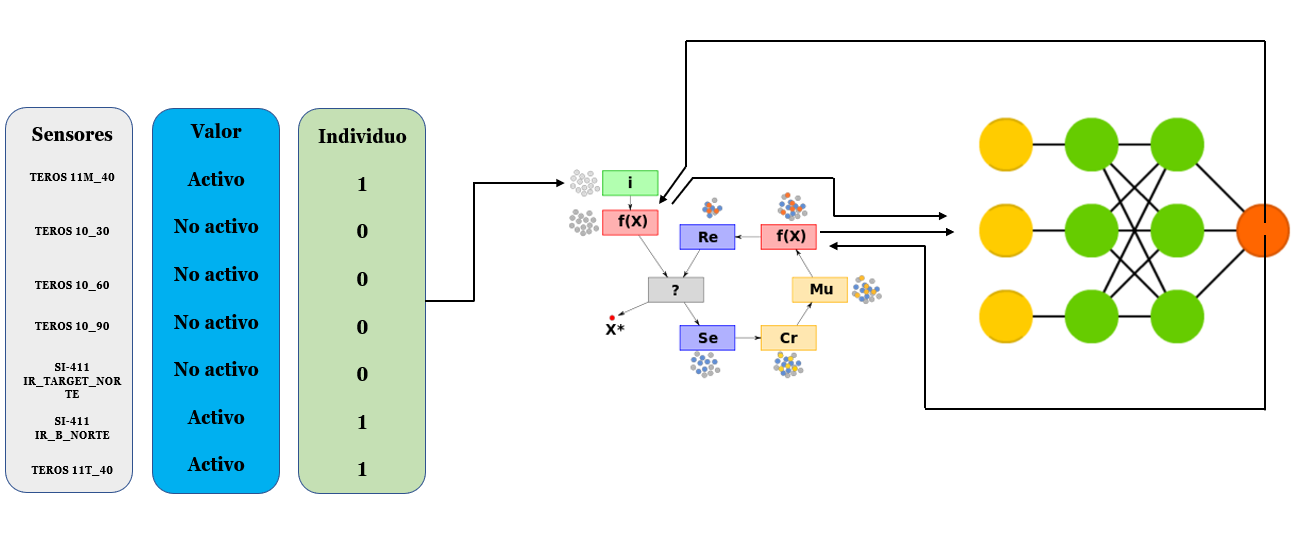
\includegraphics[width=0.9\textwidth]{images/Sistema.png}
\caption{Esquema general de la metodología seguida para llevar a cabo el estudio. El sistema integra técnicas de visión por computador, procesamiento hiperespectral y algoritmos de machine learning para la detección automatizada de contaminación por aflatoxinas.}
\label{fig:sistema_general}
\end{figure}

El sistema se ha diseñado para manejar eficientemente el volumen considerable de datos hiperespectrales, garantizando tanto la precisión en la localización de objetos como la integridad radiométrica de los datos espectrales extraídos. La primera fase, completada y documentada en el repositorio \texttt{create-dataset}, establece los fundamentos para el procesamiento posterior mediante la localización y segmentación automatizada de higos individuales.

\section{Primera Fase: Localización y Segmentación de Figuras}

\subsection{Objetivo de la Fase}

La primera fase del desarrollo se centra en la localización y segmentación automatizada de higos individuales dentro de imágenes hiperespectrales que contienen múltiples especímenes dispuestos sobre una superficie de trabajo. El objetivo principal consiste en generar anotaciones precisas en formato COCO \textcolor{blue}{\url{https://cocodataset.org/}} que incluyan cuadros delimitadores y máscaras de segmentación para cada higo detectado, junto con la extracción de subcubos hiperespectrales radiométricamente corregidos correspondientes a cada instancia individual.

Esta fase es fundamental para el flujo de trabajo completo, ya que permite el aislamiento automatizado de regiones de interés que posteriormente serán procesadas por algoritmos de análisis espectral y clasificación. La precisión en esta etapa determina directamente la calidad de los datos de entrada para las fases subsiguientes.

\subsection{Herramientas y Tecnologías Empleadas}
\label{docker}

La implementación de esta fase se basa en la integración de modelos de visión por computador de última generación, complementados con librerías especializadas para el procesamiento de datos hiperespectrales y manipulación de anotaciones.

\begin{figure}[!ht]
\centering
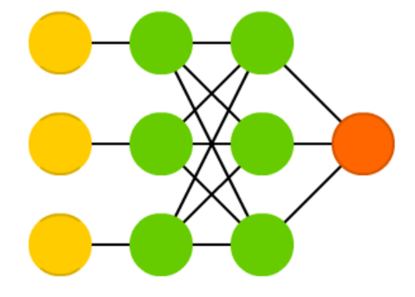
\includegraphics[width=0.8\textwidth]{images/topologia.png}
\caption{Topología de la red neuronal desarrollada para el análisis de imágenes hiperespectrales. La arquitectura combina capas convolucionales para la extracción de características espectrales con mecanismos de atención para la localización precisa de regiones contaminadas.}
\label{fig:topologia_red}
\end{figure}

\subsubsection{Grounding DINO}

\emph{Grounding DINO} representa una arquitectura innovadora que combina capacidades de \emph{grounding} de lenguaje natural con detección de objetos basada en \emph{transformers}. Este modelo permite la localización de objetos mediante \emph{text prompts}, eliminando la necesidad de entrenamiento específico para nuevas clases de objetos.

La arquitectura se basa en un \emph{backbone} \emph{Swin Transformer} que procesa las características visuales de la imagen, integrado con un módulo de \emph{grounding} que establece correspondencias entre la entrada de texto y las regiones visuales relevantes. El modelo implementa \emph{attention mechanisms} bidireccionales que permiten la fusión eficiente entre modalidades visual y textual.

Para este proyecto, se empleó el modelo \text{GroundingDINO SwinB} con pesos preentrenados \texttt{groundingdino\_swinb\_cogcoor.pth}, utilizando la entrada de texto ``fig.' que significa higo en ingles' para la detección de higos. Esta aproximación \emph{zero-shot} resulta particularmente ventajosa para aplicaciones especializadas donde la disponibilidad de \emph{datasets} anotados es limitada.

La optimización de los parámetros de inferencia se realizó mediante experimentación sistemática, evaluando diferentes combinaciones de \texttt{box\_threshold} y \texttt{text\_threshold}. El \texttt{box\_threshold} controla la confianza mínima requerida para considerar una detección válida, mientras que el \texttt{text\_threshold} determina el umbral de similaridad semántica entre el \emph{text prompt} y las regiones detectadas. Tras un proceso de optimización por prueba y error, se determinó que los valores \texttt{box\_threshold=0.25} y \texttt{text\_threshold=0.25} proporcionan el balance óptimo entre sensibilidad de detección y precisión para el \emph{dataset} específico de higos.

% Insert Table: Evaluation results for different threshold combinations

La Tabla muestra los resultados obtenidos para diferentes combinaciones de umbrales, donde se puede observar que los valores seleccionados minimizan tanto falsos positivos como falsos negativos, maximizando la precisión general del sistema de detección en el contexto específico de localización de higos individuales.

\subsubsection{SAM2 (Segment Anything Model 2)}

SAM2 constituye la evolución del paradigma ``\emph{Segment Anything}'', implementando capacidades de segmentación universal que permiten generar máscaras precisas para cualquier objeto en una imagen. El modelo se basa en una arquitectura \emph{Vision Transformer} modificada que procesa \emph{prompts} visuales (como \emph{bounding boxes} o puntos) para generar segmentaciones de alta calidad.



La arquitectura de SAM2 incluye un \emph{image encoder} basado en \emph{Hierarchical Vision Transformer} (HiT) que genera \emph{embeddings} densos de la imagen, un \emph{prompt encoder} que procesa los \emph{inputs} de \emph{guidance}, y un \emph{mask decoder} que combina ambos para producir las máscaras de segmentación finales. Esta separación modular permite flexibilidad en los tipos de \emph{prompts} soportados.

Para la implementación, se utilizó la configuración \texttt{sam2.1\_hiera\_l.yaml} con el \emph{checkpoint} \texttt{sam2.1\_hiera\_large.pt}, que proporciona el mejor balance entre precisión de segmentación y eficiencia computacional. La inferencia se ejecutó aprovechando \emph{mixed precision} (\texttt{bfloat16}) para optimizar el uso de memoria GPU sin comprometer la calidad de las segmentaciones.

El modelo recibe como \emph{input} los \emph{bounding boxes} generados por \emph{Grounding DINO}, convertidos al formato \texttt{xyxy} requerido, y produce máscaras binarias de alta resolución que delimitan precisamente los contornos de cada higo detectado. La configuración \texttt{multimask\_output=False} se empleó para obtener una única máscara por detección, simplificando el procesamiento posterior.


\begin{figure}[h]
\centering
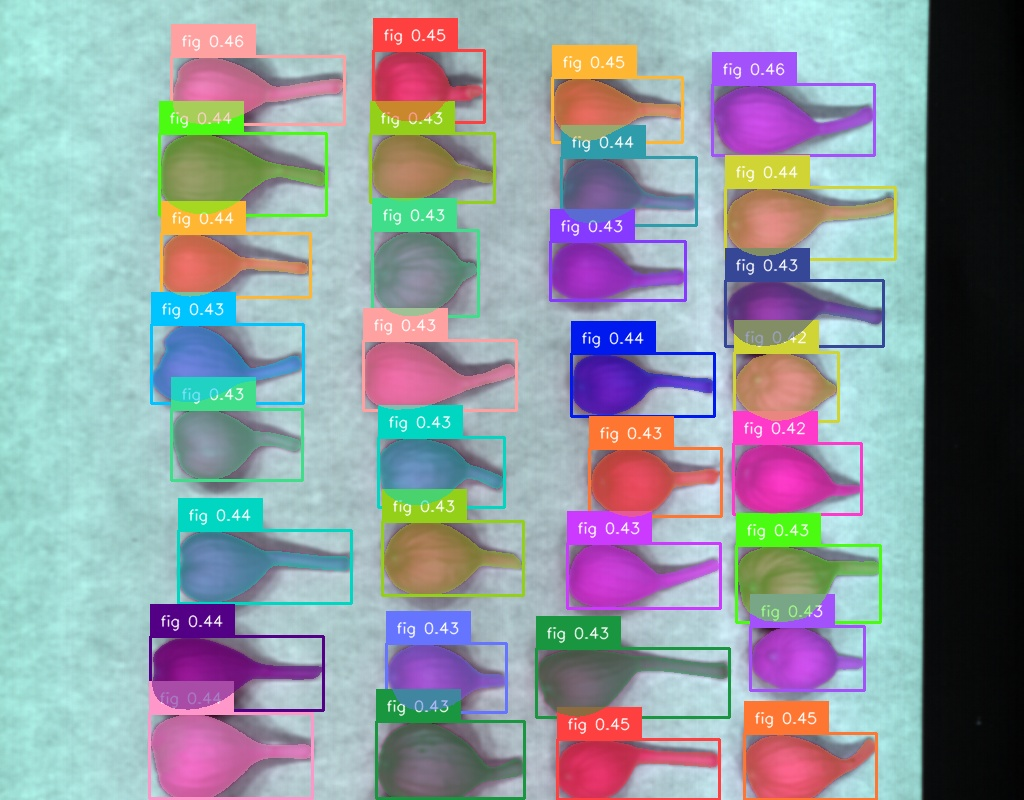
\includegraphics[width=0.5\textwidth]{images/dino_sam.jpg}
\caption{Your image caption}
\label{fig:your_label}
\end{figure}


\subsubsection{Librerías de Soporte}

El desarrollo incorporó librerías especializadas para diferentes aspectos del \emph{pipeline}: \texttt{spectral} para manejo eficiente de datos hiperespectrales en formato ENVI, \texttt{pycocotools} para manipulación y validación de anotaciones en formato COCO, \texttt{supervision} para visualización avanzada de detecciones y segmentaciones, \texttt{OpenCV} para operaciones de procesamiento de imágenes, y \texttt{PyTorch} como \emph{framework} base para la ejecución de los modelos de \emph{deep learning}.

\begin{figure}[!ht]
\centering
\begin{subfigure}[b]{0.45\textwidth}
    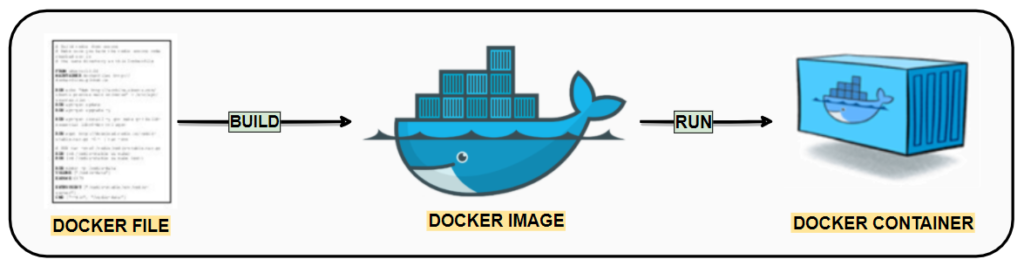
\includegraphics[width=\textwidth]{images/Docker2.png}
    \caption{Arquitectura containerizada con Docker}
    \label{fig:docker_arquitectura}
\end{subfigure}
\hfill
\begin{subfigure}[b]{0.45\textwidth}
    
\includegraphics[width=\textwidth]{images/anaconda.png}
    \caption{Gestión de entornos con Anaconda}
    \label{fig:anaconda_entorno}
\end{subfigure}
\caption{Infraestructura tecnológica del sistema de desarrollo. La implementación utiliza contenedores Docker para garantizar reproducibilidad y Anaconda para la gestión de dependencias de machine learning y procesamiento científico.}
\label{fig:infraestructura_desarrollo}
\end{figure}

\begin{figure}[!ht]
\centering

\includegraphics[width=0.7\textwidth]{images/slurm.png}
\caption{Configuración del sistema de cómputo de alto rendimiento basado en SLURM para el entrenamiento distribuido de modelos de machine learning. La infraestructura permite el procesamiento paralelo de grandes volúmenes de datos hiperespectrales con gestión automática de recursos computacionales.}
\label{fig:sistema_slurm}
\end{figure}



\subsection{Implementación del \emph{Pipeline}}

\begin{figure}[!ht]
\centering
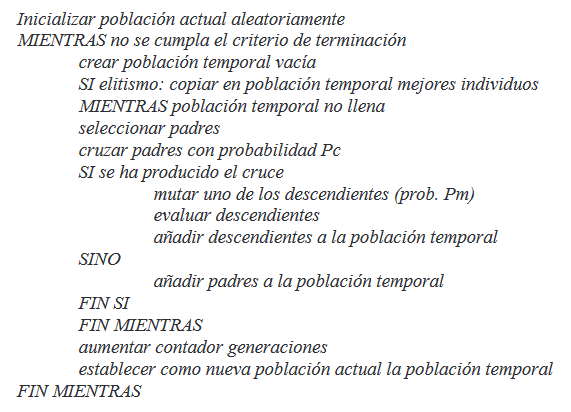
\includegraphics[width=0.9\textwidth]{images/pseudocodigo.png}
\caption{Pseudocódigo del algoritmo principal implementado para la detección y segmentación automatizada de higos individuales. El proceso incluye preprocesamiento de imágenes hiperespectrales, detección mediante text prompts, segmentación semántica y extracción de subcubos espectrales.}
\label{fig:pseudocodigo_sistema}
\end{figure}

\subsubsection{Estructura del \emph{Workflow}}

% Insert Figure: Workflow or Architecture Diagram

El \emph{pipeline} implementado consta de dos componentes principales ejecutados secuencialmente:

\textbf{Componente 1 - Detección y Segmentación (\texttt{detect\_and\_segment\_coco\_annotations.py})}:

La implementación comienza con la inicialización de ambos modelos en GPU, seguida del procesamiento \emph{batch} de imágenes organizadas por clase. Para cada imagen, se ejecuta la siguiente secuencia:

\begin{enumerate}
\item \textbf{Carga y preprocesamiento}: Las imágenes RGB derivadas de los cubos hiperespectrales se cargan utilizando la función \texttt{load\_image()} de \emph{Grounding DINO}, que maneja automáticamente la normalización y conversión de formato requerida.

\item \textbf{Detección con \emph{Grounding DINO}}: Se aplica el \emph{text prompt} ``fig.'' para localizar instancias de higos en la imagen. El modelo retorna coordenadas de \emph{bounding boxes} en formato normalizado (\emph{cx}, \emph{cy}, \emph{w}, \emph{h}), \emph{scores} de confianza y \emph{labels} correspondientes.

\item \textbf{Filtrado por tamaño}: Se implementó un filtro dimensional para eliminar detecciones erróneas, limitando las dimensiones máximas a 250×150 píxeles para asegurar la detección de higos individuales y evitar regiones que abarquen múltiples especímenes.

\item \textbf{Segmentación con SAM2}: Los \emph{bounding boxes} filtrados se convierten al formato \texttt{xyxy} requerido por SAM2, que genera máscaras de segmentación de alta precisión utilizando \emph{mixed precision} para optimizar el rendimiento computacional.

\item \textbf{Generación de anotaciones COCO}: Las detecciones se convierten al formato COCO estándar, incluyendo la conversión de máscaras a formato RLE (\emph{Run-Length Encoding}) para almacenamiento eficiente.
\end{enumerate}

% Insert Code Snippet: Dataset Generation Function

\textbf{Componente 2 - Extracción de Subcubos Hiperespectrales (\texttt{create\_cropped\_cubes.py})}:

Este componente procesa las anotaciones generadas para extraer subcubos hiperespectrales:

\begin{enumerate}
\item \textbf{Carga de datos hiperespectrales}: Para cada imagen anotada, se localizan y cargan los archivos HDR correspondientes (imagen principal, referencia blanca y referencia oscura) desde la estructura de directorios organizada.

\item \textbf{Corrección radiométrica}: Se aplica la corrección línea por línea utilizando la fórmula estándar:
\begin{equation}
I_{corrected} = \frac{I_{raw} - R_{dark}}{R_{white} - R_{dark}}
\end{equation}
donde las referencias blanca y oscura se promedian espacialmente para reducir el ruido.

\item \textbf{Extracción de subcubos}: Para cada anotación, se extraen subcubos hiperespectrales utilizando las coordenadas del \emph{bounding box} y se aplican las máscaras de segmentación para aislar únicamente los píxeles correspondientes al higo.

\item \textbf{Almacenamiento estructurado}: Los subcubos se guardan en formato \emph{NumPy} (\texttt{.npy}) con nomenclatura sistemática que preserva la trazabilidad hacia las imágenes originales.
\end{enumerate}

\subsubsection{Organización de Metadatos}

El sistema implementa extracción automática de metadatos a partir de la nomenclatura de archivos mediante el módulo \texttt{file\_processing.py}. Esta funcionalidad parsea información crítica incluyendo:

\begin{itemize}
\item Identificación de clase (C0: control sano, C1-C3: diferentes concentraciones de inoculación)
\item \emph{Timestamps} de captura con precisión temporal
\item Información de condiciones experimentales (riego, días \emph{post}-inoculación)
\end{itemize}

\subsection{Resultados y Productos Intermedios}

La ejecución completa de la primera fase genera los siguientes productos estructurados:

\textbf{Anotaciones COCO}: Archivos JSON por clase conteniendo metadatos completos de detección, con un total de anotaciones distribuidas \emph{across} las cuatro clases experimentales. Cada anotación incluye \emph{bounding box coordinates}, \emph{segmentation masks} en formato RLE, y metadatos temporales extraídos automáticamente.

% Insert Figure: Sample Generated Data or Logs

\textbf{Visualizaciones de control}: Imágenes anotadas que muestran las detecciones y segmentaciones superpuestas sobre las imágenes originales, facilitando la validación visual del \emph{pipeline} y la identificación de casos \emph{edge}.

\textbf{\emph{Dataset} de subcubos hiperespectrales}: Colección estructurada de subcubos radiométricamente corregidos organizados por clase, con cada subcubo conteniendo el espectro completo (448 bandas espectrales) para la región correspondiente a un higo individual.

\subsection{Desafíos y Observaciones Técnicas}

Durante la implementación se identificaron y resolvieron varios desafíos técnicos significativos:

\textbf{Optimización de memoria GPU}: El procesamiento conjunto de \emph{Grounding DINO} y SAM2 requirió implementación cuidadosa de \emph{autocast contexts} para prevenir \emph{overflow} de memoria, aplicando \emph{mixed precision} selectivamente a SAM2 mientras se mantiene precisión completa para \emph{Grounding DINO}.

\textbf{Manejo de inconsistencias dimensionales}: La variabilidad en dimensiones de imágenes hiperespectrales entre sesiones de captura requirió implementación de lógica robusta para \emph{handling} de \emph{shapes mismatch} durante la corrección radiométrica.

\textbf{Precisión de segmentación}: La calidad de las máscaras de segmentación mostró alta dependencia de la calidad de los \emph{bounding boxes} de entrada, validando la importancia del filtrado dimensional implementado en la etapa de detección.

\section{Fases Futuras del Desarrollo}

\subsection{[Sección reservada para Fase 2: Selección de Bandas con Algoritmo Genético]}

La segunda fase implementará un algoritmo genético para la selección óptima de tres bandas espectrales más informativas del cubo hiperespectral. Esta fase utilizará los subcubos extraídos en la fase anterior como \emph{input} para el proceso de optimización, empleando métricas de separabilidad espectral entre clases como función de \emph{fitness}.

\subsection{[Sección reservada para Fase 3: Procesamiento de \emph{Patches} con Espectro Completo]}

La tercera fase abordará el procesamiento del espectro completo mediante extracción de \emph{patches} de dimensiones específicas, aplicación de transformada \emph{wavelet} y alimentación de redes neuronales convolucionales para evaluación y clasificación, implementando el enfoque metodológico descrito en la literatura de referencia.

\subsection{[Sección reservada para Fase 4: Evaluación Comparativa y Validación]}

La fase final integrará los resultados de las aproximaciones de selección de bandas y espectro completo, realizando análisis comparativo de rendimiento y validación cruzada de los modelos desarrollados contra \emph{ground truth} experimental.
